\documentclass[11pt]{article}
\title{Technical Report\\ COMP1100 Assignment 3}
\author{Jacob Bos\\ ANU u7469354}

\usepackage{graphicx}
\usepackage{amsmath}
\usepackage{amssymb}
\usepackage{array}
	\newcolumntype{L}{>{\centering\arraybackslash}m{15cm}}
\usepackage{float}
\usepackage{multicol}
\setlength{\columnsep}{1cm}
\usepackage{setspace}
\usepackage{xcolor}

\newenvironment{smallpmatrix}
  {\left(\begin{smallmatrix}}
  {\end{smallmatrix}\right)}
 \newenvironment{smol}
  {\left(\begin{smallmatrix}}
  {\end{smallmatrix}\right)}


\usepackage[margin=2cm]{geometry}
\addtolength{\textheight}{-0.5cm}
%~~~~~~~~~~~~~~~~~~~~~~~~~~~~~~~~~~~~~~~~~~~~~~~~~~~~~~~~~~~~~~~~~~~~~~~~~~~~~~~~~~~~~~~~~~~~~~~~~~~~
%~~~~~~~~~~~~~~~~~~~~~~~~~~~~~~~~~~~~~~~~~~~~~~~~~~~~~~~~~~~~~~~~~~~~~~~~~~~~~~~~~~~~~~~~~~~~~~~~~~~~
\begin{document}
\maketitle
\pagenumbering{roman}
\setstretch{1.5}
\begin{center}
  Lab: Tuesday 11am\\
  Tutor: Abhaas Goyal\\
  Word-count beyond cover page at $\leq 1500$ words
\end{center}
\tableofcontents
\newpage
\pagenumbering{arabic}
%~~~~~~~~~~~~~~~~~~~~~~~~~~~~~~~~~~~~~~~~~~~~~~~~~~~~~~~~~~~~~~~~~~~~~~~~~~~~~~~~~~~~~~~~~~~~~~~~~~~~
\section{Introduction} 
The program detailed herein is an implementation of a few AI's for solving Fanorona with complimentary unit tests.


%~~~~~~~~~~~~~~~~~~~~~~~~~~~~~~~~~~~~~~~~~~~~~~~~~~~~~~~~~~~~~~~~~~~~~~~~~~~~~~~~~~~~~~~~~~~~~~~~~~~~
\section{Documentation}%Explanation of code workings, functions and structure.
\subsection*{Design Documentation and Technical Decisions}
% Describe what each relevant function does conceptually. (i.e. how does it get you closer to solving the problems outlined in this assignment spec?)
% How do these functions piece together to make the finished program? Why did you design and implement it this way?
% What major design choices did you make regarding the functions that you’ve written and the overall structure of your program?
\paragraph*{First capture move,} used to test the greedy AI, is an AI that takes the head a list of possible capturing moves provided by \verb|captures| else returning the first legal move.

\paragraph{The Greedy AI} is conceptually simple. The main function \verb|greedy| cases on the turn in the gamestate and picks the move that either maximizes (for Player1) or minimizes (Player2) the heuristic value. It does this using \verb|greedyHelp| that recurses through a list of move/value pairs using an accumulator and the appropriate evaluator to pick the move. This move/value list is generated by a mapping of \verb|diffPieces| and \verb|applyMove| to the \verb|legalMoves| list.

\paragraph{The first Minimax} uses two trees, \verb|GameTree| stores all the possible gamestate evolutions and is generated through an infinite recursion in \verb|gameTree| which takes a state, puts it into a node and then maps \verb|gameTree| to all its child states generated through a mapping of \verb|applyMove| to a list of \verb|legalMoves| which has \verb|Nothing|s recursively filtered out by \verb|purge|.

\subparagraph*{}\verb|EvalTree| is similar to \verb|GameTree| but stores a value corresponding to the best possible heuristic value for the player who's turn it is at a node, and is pruned to a given \textit{move depth}. The \verb|EvalTree| is generated by \verb|pruneMinMax| recursively navigating the \verb|GameTree|, casing on the depth given to the function, if the depth is zero or the game is over then it evaluates the heuristic value at that node and then terminates that branch. Else, it cases on the state held in the node. If the state at a node contains \verb|Turn Player1| then it assigns the maximum of the values in its child \verb|EvalTree| nodes else if the turn is the \verb|Player2| it assigns the minimum value of its child nodes to the given node. This results in the best possible outcome for the player in the initial state ending up in the head node. The heuristic value, calculated by \verb|heuristicVal|, is the difference in the number of pieces between players given by \verb|countPieces|.

\subparagraph*{}To retrieve the best move we note that the best move is at the same depth in the \verb|legalMoves| list as the value stored in the head node is in the list of child nodes. This is because the list of child nodes is produced by a mapping on the \verb|legalMoves| list. Consequently to find the best move, we extract the value from the head node of the output of \verb|pruneMinMax| using \verb|getVal| and then find its depth recursively using \verb|findDepth| in the list provided by mapping \verb|getVal| to the child nodes. Consequently \verb|getMove| uses (!!) to extract the best move at its expected depth in the \verb|legalMoves| list.

\paragraph*{The second Minimax} Is identical to the first except that the heuristic function assigns win or loss gamestates with values more extreme than typical. Doing so improved performance by a little, weighting winning more heavily.

\subsection*{Program Design}
The AI structures are graphed below:
\begin{center}
  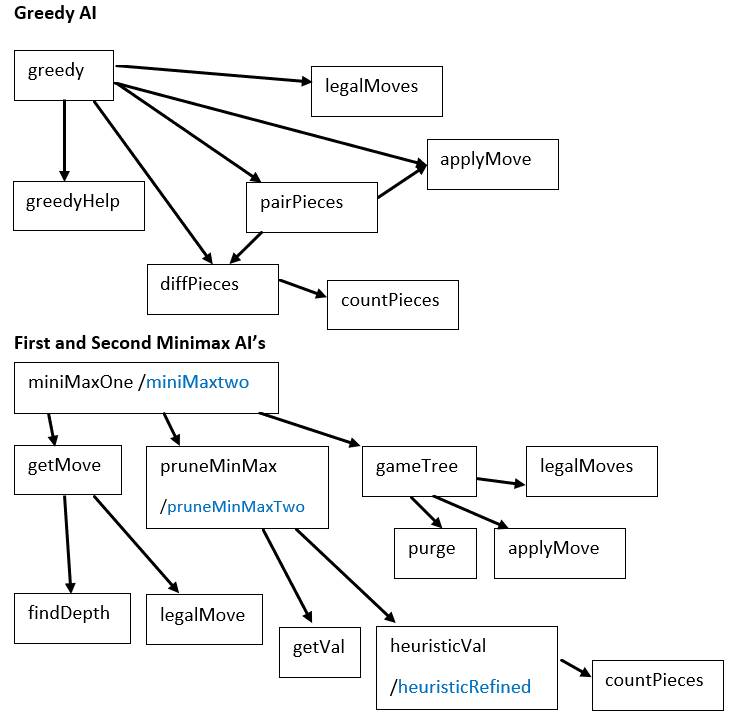
\includegraphics[width=0.85\textwidth]{functDep.png}
\end{center}

\paragraph{The Greedy AI} currently does a lot of unnecessary work with Maybe types which could be eliminated with the strategies used in the minimax AIs that were later developed. The maybe types used require extra case statements and so it was necessary to break the AI into a number of helpers to improve readability.

\paragraph{Both MiniMax AIs} share the same structure and most of their functions. Both are called by a top end function that inputs the initial state and calls a function that gets the move based on the result of the pruner function's evaluation tree. It was chosen to move \verb|getVal| to a helper function to reduce the population of things in the pruner's \verb|where| clause.

 \subsection*{Assumptions}%Describe assumptions you have made about how a user might use the program and how this has influenced your design decisions.
The primary assumption made is that the ordering of the \verb|legalMoves| list is the same as the ordering of their values in the child nodes of \verb|EvalTree|. This assumption is reasonable because there should be no \verb|Nothing|s in the list for \verb|purge| to remove because they result from an illegal move being fed to \verb|applyMove| which is impossible using \verb|legalMoves|. Thus the values in the first child nodes are just repeated mappings onto the \verb|legalMoves| list, preserving order. %A second assumption made was that the \verb|legalMoves| list would never be empty because this would be prohibited by the game ending at that point. Consequently it was acceptable for \verb|findDepth| to return an error for an empty list.

%~~~~~~~~~~~~~~~~~~~~~~~~~~~~~~~~~~~~~~~~~~~~~~~~~~~~~~~~~~~~~~~~~~~~~~~~~~~~~~~~~~~~~~~~~~~~~~~~~~~~
\newpage
\section{Testing}%How did I test the program focus on methodology and testing groups
%How did you test individual functions?
%Be specific about this - the tutors know that you have tested your program, but they want to know how.
%Describe the tests that prove individual functions on their own behave as expected (i.e. testing a function with different inputs and doing a calculation by hand to check that the outputs are correct).
%How did you test the entire program? What tests did you perform to show that the program behaves as expected in all (even unusual) cases?
\paragraph{Unit tests} aimed to cover as many cases on as many functions as possible. Unfortunately, many of the functions deal with complex datatypes made writing typical arguments difficult. Consequently some tests use \verb|initialState| and compare the lengths of arguments and outputs.

\subparagraph{The Greedy AI} has two test groups. \verb|pairPieces| was tested by checking that the list of pairs of legal moves and their associated heuristic value is the same length as the list of \verb|legalMoves|. The passing of this test asserts the function's correctness. \verb|diffPieces| is tested against two cases, that it returns \verb|Nothing| for argument \verb|Nothing| and \verb|Just 0| for an argument of just \verb|initialState|.

\subparagraph{The MiniMax AI} has four test groups. Firstly \verb|purge| has four test cases. They were made easier to write because \verb|purge| is polymorphic and so a simpler input type of \verb|Int| was used. \verb|purge| is then tested against a case of the empty list, all \verb|Nothing|s, all \verb|Just x|'s and a mix of \verb|Nothing|s and \verb|Just|s. Passing these tests implied that the function was correct. Similarly, since \verb|findDepth| is polymorphic it was easier to write test cases. It was not tested against the empty list since that returns an error but was tested against cases where the element occurred once or twice in the list where its supposed to take the first. Thirdly, \verb|getVal| was tested against one test case, indicating its ability to correctly retrieve a nodes's value. Lastly \verb|heuristicVal| was tested with the initial state as an argument to ensure that the output is zero as would be expected. Unfortunately it was difficult to test it against any other inputs as other arguments are difficult to write.

\paragraph{Performance tests} were done by playing my AIs against themselves and the tournament's course AIs.

The correctness of the Greedy AI was confirmed by it beating both \verb|firstlegalMove| and \verb|firstCaptureMove| as it should statistically behave better than both. Whilst a faulty Greedy may be able to beat FLM by chance it is less likely to beat an FCM by chance especially if it was accidentally minimizing when it was supposed to maximize or vices-versa. Since the Greedy was also able to consistently beat me as a human I considered that it was likely correct.

\subparagraph{The MiniMax AI's} were tested against both the greedy AI and the Course AIs, \verb|miniMaxtwo| consistently outperformed \verb|greedy| and all of the course greedy AIs except for third where playing first results in a draw. \verb|MiniMaxTwo| majority draws against the course Minimaxes and Alpha-beta pruners further indicating correctness. It would be expected with such a simple heuristic that another minimax or minimax-alpha/beta AI with a better heuristic would slightly outperform. 

%~~~~~~~~~~~~~~~~~~~~~~~~~~~~~~~~~~~~~~~~~~~~~~~~~~~~~~~~~~~~~~~~~~~~~~~~~~~~~~~~~~~~~~~~~~~~~~~~~~



\newpage
\section{Reflection}
%Discuss the reasoning behind your decisions, rather than what the decisions were. You can reflect on not only the decisions you made, but the process through which you developed the final program:
  %What would you have done differently if you were to do it again
    %What changes to the design and structure you would make if you wrote the program again from scratch?
  \subsection*{Design Choices}
  For \verb|greedy| and \verb|miniMaxOne| it was decided to use the difference of pieces as the heuristic due to its easy implementation using \verb|countPieces| from \verb|Fanorona.hs|. This was done to allow greater time to design and understand the algorithms. The second Minimax used the updates described in an attempt to prioritize winning moves in endgame. It was chosen that the greedy AI should pair moves with their associated value to allow for an accumulator recursion to find the move with the best outcome. In contrast the minimax AI's did not store moves in the structure, relying on the discussed assumption about list lengths. This was done in order to simplify the structures and functions as much as possible in an attempt to improve style and speed, being able to use pre-optimized functions like \verb|maximize| and avoid convoluted datatypes. The minimax pruners were designed to make as good use of laziness as possible. This allowed a node to be assigned the minimum of maximum value of its children before the children were evaluated. The structure of each AI was dictated by the authors thought process and the ideas that came to them. Functions were refined in the ways that the author felt were suitable and enhanced style.

  \subsection*{Reflection}
  Upon reflection the author would have designed the pruner to take a heuristic function as an argument so as to not need to rewrite the pruner function to implement a different heuristic. Further, they would have removed the states from the nodes of the \verb|EvalTree| to simplify the structure. It would be beneficial to implement a pruning strategy such as alpha-beta to increase the possible search depth. Also, time would be spent developing a heuristic based on a deeper understanding of the game to evaluate the worth of different arrangements of pieces. Unfortunately they had no time to invest in developing an alpha-beta pruner and struggled to decide how to modify the current pruning function, undecided as to whether keep track of the values in the \verb|evalTree| or accumulated in the pruner function's arguments.


%~~~~~~~~~~~~~~~~~~~~~~~~~~~~~~~~~~~~~~~~~~~~~~~~~~~~~~~~~~~~~~~~~~~~~ ~~~~~~~~~~~~~~~~~~~~~~~~~~~~~~~


%~~~~~~~~~~~~~~~~~~~~~~~~~~~~~~~~~~~~~~~~~~~~~~~~~~~~~~~~~~~~~~~~~~~~~~~~~~~~~~~~~~~~~~~~~~~~~~~~~~~~
\end{document}
